\documentclass[a4paper,11pt, twoside]{report}
\usepackage{hyperref}
\usepackage{graphicx}
\usepackage{caption}
\usepackage[]{newfloat}

\begin{document}

\section*{Relazione progetto High-performance Computing}
\subsection*{Michele Ceccacci, mat. 0001027124}
\subsubsection*{\today}

\subsection*{Introduzione}
L' obiettivo di questa relazione è parallelizzare il programma circles.c usando openMP e MPI. 
Questo programma calcola prende cerchi sovrapposti e li sposta minimizzando le loro sovrapposizioni.
Ho usato la funzionalità movie per verificare la correttezza di entrambe le implementazioni in maniera visuale. 
Inoltre ho cercato di vedere se il codice esempio non parallelizzato avesse un numero di overlap simili al codice MPI e OMP a ogni iterazione.
Ho cercato di sfruttare il fatto che il programma MPI non ha race condition per cercare race condition nella versione OMP.
Infatti, dato che i thread condividono lo stesso address space, questo potrebbe risultare in race condition. 
L' approccio usato per entrambi i programmi paralleli è stato quello di cercare di ottenere codice corretto,e poi parallellizzarlo e guadagnare più performance possibile.
L' unica funzione che presenta loop-carried dependencies nel codice seriale è \textit{move\_circles}.
\subsection*{Versione OpenMP}
Parallelizzato usando \textbf{openMP}.
Ho deciso di estrarre i delta x e y nella struttura circle in array separati, così da poterli usare insieme alla primitiva \textit{OpenMP reduce}.
Nella funzione reduce\_forces, ho parallellizzato solo il loop esterno, che non presenta nessuna loop-carried dependency.
Dato che il workload è molto sbilanciato e le performance non erano ottimali, ho poi deciso di usare scheduling dinamico.
Ho usato il costrutto openMP parallel for, e ho definito le variabili con default(none), in maniera da dover pensare al significato di ogni singola variabile e non lasciare ambiguità nel mio codice.
Ho definito variabili che non vengono modificate come shared per evitare copie inutili.
Inoltre ho sempre usato il costrutto reduce di openMP per computare le somme sia degli offset che della variabile che rappresenta il numero di sovrapposizioni.
Questo mi ha consentito di evitare race condition, e di rendere il mio codice più semplice senza impattare in alcun modo la performance.
\begin{figure}
    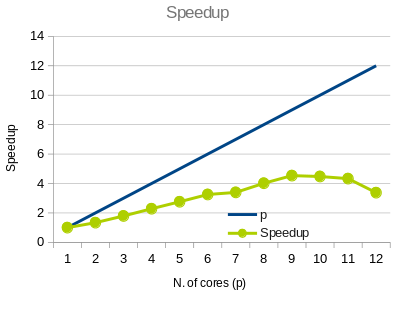
\includegraphics[scale=0.5]{images/omp_speedup.png}
    \caption[]{Lo speedup misurato del programma \textit{omp\_circles} è quasi lineare}
\end{figure}
\begin{figure}
    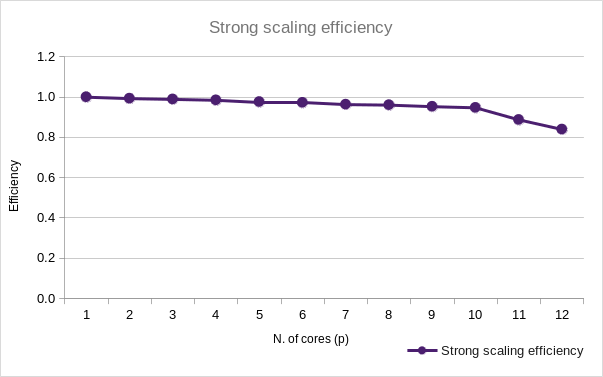
\includegraphics[scale=0.5]{images/omp_strong.png}
    \caption[]{La strong scaling efficiency rimane vicina a 1 con numero di thread minore o uguale a 10 per poi diminuire leggermente}
\end{figure}
La ragione per cui lo speedup diminuisce nella dodicesima iterazione è che il thread probabilmente viene usato dal sistema operativo.
Dato che il carico è bilanciato dinamicamente, ogni thread prende una frazione del lavoro uguale agli altri, 
e le performance in weak scaling sono molto buone.
\begin{figure}
    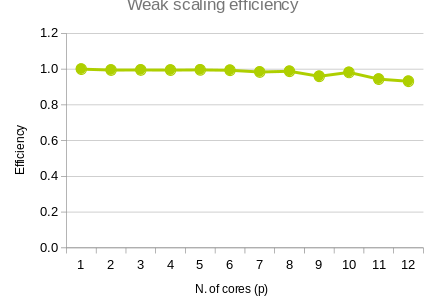
\includegraphics[scale=0.5]{images/omp_weak.png}
    \caption[]{Le performance in weak scaling sono molto buone, rimanendo sempre vicine a 1}
\end{figure}
\section*{Versione MPI}
Usando \textbf{MPI}, dato che ogni processo ha bisogno di ricevere un' array aggiornato con tutte le informazioni rilevanti ai cerchi, 
ho dovuto definire un nuovo data type circle, che ho potuto usare per inviare direttamente le informazioni. 
Questo mi consente di ridurre il numero di \textbf{MPI\_Bcast} necessarie ad ogni iterazione.
Dato che a ogni processo servono le informazioni presenti in tutto l' array, e non solo una porzione, ho usato \textbf{MPI\_Bcast} per facilitare l' invio e non duplicare lavoro,
che sarebbe successo se avessi scelto di usare \textbf{MPI\_send} o  \textbf{MPI\_recv}.
Dopo aver calcolato i nuovi displacement sull'asse x e y, ho usato \textbf{MPI\_reduce}. 
In questo caso ho preferito codice piu semplice al definire una operazione di reduce custom,
che permette efficienza migliore rispetto all' usare direttamente primitive di livello più basso.
Per bilanciare il carico, ho modularizzato il codice e fatto in modo che lo stesso thread che calcola i displacement per il cerchio $i$ lo calcoli anche per il cerchio $n-i$.
Questo risulta nel fatto che a ogni iterazione $i$ del ciclo da $0$ a $\frac{n}{2}$, il lavoro fatto rimane costante, dato che il lavoro fatto a ogni iterazione è $i + (n-i) = n$.
A questo punto, se un processo itera sullo stesso numero di coppie di cerchi, allora compie lo stesso lavoro di un altro, qualunque sia il suo indice $i$.
Inoltre, ho deciso di usare la funzione reset\_displacement direttamente al posto di mandare il buffer con displacement resettati a 0.
Questo consente di limitare le comunicazioni inter-process necessarie.
\begin{figure}
    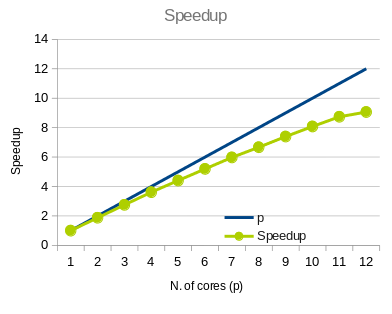
\includegraphics[scale=0.5]{images/mpi_speedup.png}
    \caption[]{Lo speedup rimane molto vicino a lineare con un numero di processi minore o uguale a 10, per poi calare con 11 e 12 processi}
\end{figure}
\begin{figure}
    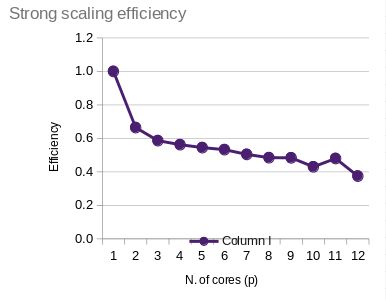
\includegraphics[scale=0.5]{images/mpi_strong.png}
    \caption[short]{La performance in strong scaling rimane vicino a 1 fino a quando si usano 10 processi, e cala fino a 0.8 con 12 processi}
\end{figure}
\begin{figure}
    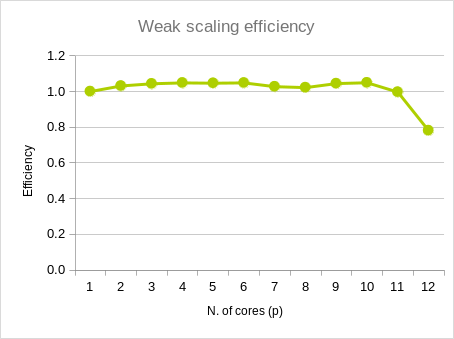
\includegraphics[scale=0.5]{images/mpi_weak.png}
    \caption[short]{La performance in weak scaling rimane vicino a 1 fino a quando si usano 10 processi, e cala fino a 0.8 con 12 processi} 
\end{figure}
\newline
La ragione per cui lo speedup diminuisce nella dodicesima iterazione è che il thread probabilmente viene usato dal sistema operativo.
\section*{Conclusioni}
Ho ottenuto uno speedup significativo sia nella versione MPI che nella versione OpenMP.
La differenza principale tra il programma MPI e il programma OpenMP è la mancanza di dynamic scheduling nella versione MPI.
Questo è stato risolto bilanciando il carico in modo manuale nella versione MPI.
Un'altra possibile ottimizzazione è aumentare la cache locality iterando sui displacement x e y separatamente.
Questo consente al programma di dover tenere nella cache solo il displacement corrente, effettivamente raddoppiando il numero di displacement nella cache.
Ho inoltre notato che il numero di intersezioni non sono esattamente uguali tra versione parallellizzata e seriale, ma differiscono di circa lo 0.5\% alla ventesima iterazione.
Dopo una sessione di debugging, credo che questo sia dovuto al fatto che i float che rappresentano i displacement vengono sommati in un ordine diverso, dando origine così a risultati leggermente inconsistenti.

\end{document}
